\documentclass[a4paper,11pt]{extarticle}
\usepackage[a4paper]{geometry}
\geometry{verbose,tmargin=2cm,bmargin=2cm,lmargin=2cm,rmargin=2cm}

%\usepackage{graphicx}

\usepackage{fontspec}
\setmonofont{FreeMono}

\setlength{\parindent}{0cm}
\setlength{\parskip}{0.5em}

\usepackage{textcomp}

\usepackage{hyperref}
\usepackage{url}
\usepackage{xcolor}

\usepackage{minted}
\newminted{cpp}{breaklines,fontsize=\small}
\newminted{gnuplot}{breaklines,fontsize=\small}
\newminted{text}{breaklines,fontsize=\small}

\definecolor{mintedbg}{rgb}{0.95,0.95,0.95}
\usepackage{mdframed}

\BeforeBeginEnvironment{minted}{\begin{mdframed}[backgroundcolor=mintedbg]}
\AfterEndEnvironment{minted}{\end{mdframed}}

\title{
MI2101\\
Praktikum Teknik Komputasi\\
Modul 2}
\author{Fadjar Fathurrahman}
\date{2018}

\begin{document}
\maketitle

\section{Tujuan}
\begin{itemize}
\item Mampu membuat program C++ sederhana dengan percabangan dan perulangan
\item Mampu membuat program C++ yang menangani input sederhana dari penggunan
\item Membuat data plot dengan program eksternal seperti \textsf{Microsoft Excel},
\textsf{Libre Office Calc} dan \textsf{Gnuplot}
\end{itemize}

\section{Perangkat lunak yang diperlukan}
\begin{itemize}
\item Linux OS
\item CodeBlocks yang telah dikonfigurasi untuk kompiler GNU C/C++
\item Terminal emulator dengan \texttt{bash} sebagai shell (baris perintah)
\item Editor teks seperti \texttt{gedit}
\item Perangkat lunak untuk membuat plot/grafik:
\begin{itemize}
\item Spreadsheet program seperti \textsf{Microsoft Excel} atau \textsf{Libre Office Calc}
\item \textsf{Gnuplot}
\end{itemize}
\end{itemize}

\section{Akar persamaan kuadrat}
Pada modul sebelumnya kita telah membuat program sederhana untuk menghitung
akar-akar dari persamaan kuadrat
\begin{equation}
ax^2 + bx + c = 0
\label{eq:pers_kuadrat}
\end{equation}
$a, b, c$ adalah bilangan real, dengan batasan bahwa $D = b^2 - 4ac >= 0$.
Pada bagian ini, kita akan memperbaiki program sebelumnya dengan
membolehkan kasus $D < 0$. Pada kasus ini, akar-akar dari persamaan
\ref{eq:pers_kuadrat} dapat dinyatakan sebagai:
\begin{equation}
x_{1,2} = -\frac{b}{2a} \pm \frac{\sqrt{-D}}{2a}\imath
\end{equation}
Dari persamaan di atas dapat dilihat bahwa $x_{1}$ dan $x_{2}$ adalah
pasangan konjugat kompleks.

\subsection{Tugas: akar-akar real dan imajiner}

Buatlah program untuk menghitung akar-akar dari persamaan kuadrat
seperti pada Modul 1, namun juga memperhitungkan kasus diskriminan negatif
(akar-akar kompleks).
Anda dapat menggunakan konstruksi \texttt{if-else} pada C++.
Program berikut ini dapat Anda lengkapi sebagai panduan.

\begin{cppcode}
#include <iostream>
#include <cmath>

using namespace std;

int main()
{
  float a, b, c;
  // berikan nilai a, b, dan c di sini
  a = ...;
  b = ...;
  c = ...;
  // Tampilkan pesan ke layar
  cout << "Mencari akar-akar persamaan kuadrat" << endl;
  cout << endl;
  cout << "a*x^2 + b*x + c = 0" << endl;
  cout << endl;
  cout << "a = " << a << endl;
  cout << "b = " << b << endl;
  cout << "c = " << c << endl;
  cout << endl;
  // Hitung diskriminan di sini
  float D;
  D = ....;
  // Tampilkan nilai diskriminan
  ....
  // Deklarasi variabel
  ....
  if( D >= 0.0 ) { // akar real
    x1 = ....;
    x2 = ....;
    cout << "Akar-akar real:" << endl;
    .... // tampilkan x1 dan x2
  }
  else { // akar imajiner
    ....
    cout << "Akar-akar imajiner:" << endl;
    ....
  }
  return 0;
}
\end{cppcode}

Contoh keluaran program di atas untuk kasus akar-akar real.
\begin{textcode}
Mencari akar-akar persamaan kuadrat

a*x^2 + b*x + c = 0

a = 2
b = 1
c = -4

D = 33

Akar-akar real:

x1 = 1.18614
x2 = -1.68614
\end{textcode}

Contoh keluaran program di atas untuk kasus akar-akar imajiner.
\begin{textcode}
Mencari akar-akar persamaan kuadrat

a*x^2 + b*x + c = 0

a = 2
b = 1
c = 4

D = -31

Akar-akar imajiner:

x1 = -0.25 + 1.39194i
x2 = -0.25 - 1.39194i
\end{textcode}


\subsection{Tugas: akar persamaan kuadrat dengan input dari pengguna}

Modifikasi program pada tugas sebelumnya agar dengan membaca input
nilai $a, b, c$ dari pengguna secara interaktif. Anda
dapat menggunakan pernyataan \texttt{cin} pada C++.

Contoh keluaran dari program:
\begin{textcode}
Masukkan nilai a: 1.0
Masukkan nilai b: 2.1
Masukkan nilai c: 8.0

Mencari akar-akar persamaan kuadrat

a*x^2 + b*x + c = 0

a = 1
b = 2.1
c = 8

D = -27.59

Akar-akar imajiner:

x1 = -1.05 + 2.62631i
x2 = -1.05 - 2.62631i
\end{textcode}


\section{Perulangan}
Dalam bagian ini, kita akan latihan menggunakan konstruksi perulangan \texttt{for}
untuk melakukan perhitungan berulang. Pada contoh berikut ini dan beberapa
latihan berikutnya kita akan mempersiapkan data tabular yang akan diplot
dengan menggunakan \textsf{Gnuplot}. Anda tentu saja dapat menggunakan program
lain seperti \textsf{Microsoft Excel} atau \textsf{Libre Office Calc}.

Berikut ini adalah contoh program yang akan digunakan untuk menghasilkan data.
Misalkan nama file yang digunakan adalah \texttt{DataSinCos.cpp}.
\begin{cppcode}
#include <cstdio>
#include <cmath>
int main()
{
  int i;
  double x, y1, y2;
  int NptsPlot = 10;
  const double xi = 0.0;
  const double xf = 1.0;
  const double L = xf - xi;
  double delta_x = L/(NptsPlot-1);
  for(i = 0; i < NptsPlot; i++) {
    x = xi + i*delta_x;
    y1 = sin(2.0*M_PI*x/L);
    y2 = cos(2.0*M_PI*x/L);
    printf("%18.10f %18.10f %18.10f\n", x, y1, y2);
  }
  return 0;
}
\end{cppcode}

Beberapa catatan mengenai kode di atas adalah sebagai berikut.
\begin{itemize}
\item Tipe data \texttt{double} digunakan agar hasil perhitungan lebih teliti.
\item Penggunaan fungsi \texttt{printf} dan \texttt{\#include <cstdio>}
\item Konstanta \verb|M_PI| digunakan sebagai bilangan $\pi$
\end{itemize}

Contoh keluaran dari program ini adalah sebagai berikut.
\begin{textcode}
      0.0000000000       0.0000000000       1.0000000000
      0.1111111111       0.6427876097       0.7660444431
      0.2222222222       0.9848077530       0.1736481777
      0.3333333333       0.8660254038      -0.5000000000
      0.4444444444       0.3420201433      -0.9396926208
      0.5555555556      -0.3420201433      -0.9396926208
      0.6666666667      -0.8660254038      -0.5000000000
      0.7777777778      -0.9848077530       0.1736481777
      0.8888888889      -0.6427876097       0.7660444431
      1.0000000000      -0.0000000000       1.0000000000
\end{textcode}

Anda dapat mencoba membuat plot dari data ini dengan cara mengkopi output tersebut
ke program spreadsheet.
Alternatif yang akan kita gunakan pada praktikum ini adalah dengan menggunakan
program \textsf{Gnuplot}.

Misalkan nama program hasil kompilasi adalah \texttt{DataSinCos}.
Anda dapat melakukan \textit{redirection} output program ke suatu file
dengan nama
\begin{textcode}
./DataSinCos > sin_cos.dat
\end{textcode}

\textsf{Gnuplot} adalah program berbasis terminal. Program ini dapat dijalankan
secara interaktif maupun non-interaktif melalui file \textit{script}.
Dalam praktikum ini kita
akan lebih banyak menggunakan mode non-iteraktif dengan menggunakan \textit{script}

Buat file berikut ini dengan menggunakan teks editor seperti \textsf{Gedit}
dan simpanlah dengan name \texttt{do\_plot\_sin\_cos.plt}.
\begin{gnuplotcode}
set terminal pdf font "Times New Roman, 14"
set output "sin_cos.pdf"
set xlabel "x"
set ylabel "y"
set title "sin(x) dan cos(x)" # judul plot
set key at 0.6,1.0 # Posisi legenda
set xrange [-0.1 : 1.1]
set yrange [-1.1 : 1.1]
plot "sin_cos.dat" using 1:2 with linespoints title "sin(x)" \
                   pointtype 7 pointsize 0.5,\
                "" using 1:3 with linespoints title "cos(x)" \
                   pointtype 7 pointsize 0.5,
\end{gnuplotcode}
Anda dapat membaca lebih banyak mengenai arti perintah tersebut pada
manual \textsf{Gnuplot} yang dapat ditemukan pada laman
\textsf{Gnuplot} \url{http://gnuplot.sourceforge.net/}.

Panggil \textsf{Gnuplot} untuk menjalankan script \texttt{do\_plot\_sin\_cos.plt}.
\begin{textcode}
gnuplot do_plot_sin_cos.plt
\end{textcode}

Hasil plot tersebut dapat dilihat pada gambar berikut.

{\centering
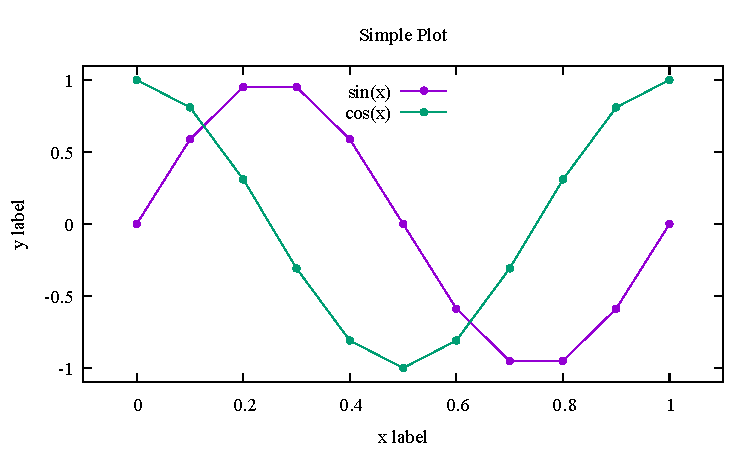
\includegraphics[scale=1.0]{sin_cos.pdf}
\par
}

Untuk mendapatkan plot yang lebih halus (\textit{smooth}) kita dapat menggunakan
parameter \texttt{NptsPlot} yang relatif besar misalnya 200 dan disesuaikan juga
dengan rentang nilai $x$ di mana fungsi diplot.


\subsection{Tugas: Plot fungsi eksponensial}

Buat program seperti di atas untuk fungsi Gaussian berikut ini.
\begin{equation}
f(x) = \frac{1}{\sigma\sqrt{2\pi}}\exp\left(-\frac{(x-\mu)^2}{2\sigma^2}\right)
\end{equation}
dengan $\sigma > 0$ dan $\mu$ merupakan dua parameter.
Buatlah plot dua fungsi Gaussian
dengan parameter masing-masing sebagai berikut:
$(\mu_{1}=1.0,\sigma_{1}=1.5)$ dan $(\mu_{2}=-2.0,\sigma_{2}=1.0)$.
Hasil plot tersebut dapat dilihat pada gambar berikut.

{\centering
\includegraphics[scale=1.0]{TEMP_normal_gaussian.pdf}
\par}

Anda dapat menggunakan fungsi \texttt{exp} dari \texttt{cmath}
untuk menghitung eksponensial.

\subsection{Tugas: Plot fungsi sinc}
Lakukan sesuai dengan tugas sebelumnya namun untuk fungsi berikut ini:
\begin{equation}
f(x) = \mathrm{sinc}(x) = \frac{\sin(\pi x)}{\pi x}
\end{equation}
Buat plot fungsi $\mathrm{sinc}(x)$ pada rentang $-10 < x < 10$
dan dengan menggunakan \texttt{NptsPlot} bilangan ganjil, misalnya 201.
Bagaimana dengan nilai $\mathrm{sinc}(x=0)$ ?

{\centering
\includegraphics[scale=1.0]{TEMP_sinc.pdf}
\par}

\section{Tugas/Pekerjaan rumah}

\begin{enumerate}
\item Tinjau kembali program untuk mencari akar-akar persamaan kuadrat dengan input
$a, b, c$ dari pengguna. Ketika diminta untuk memasukkan nilai-nilai tersebut,
coba masukkan input yang tidak valid (bukan angka) misalnya huruf \texttt{a}.
Apa yang terjadi ?
Jika terjadi kesalahan bagaimana cara memperbaikinya ?
%
\item Buatlah visualisasi untuk ekpansi deret Fourier berikut ini.
  \begin{enumerate}
  %
  \item Gelombang segitiga
  \begin{equation}
  f(x) = \frac{8}{\pi^2} \sum_{n=1,3,5,\ldots}^{\infty}
  \frac{(-1)^{(n-1)/2}}{n^2}\sin\left( \frac{n\pi x}{L} \right)
  \end{equation}
  %
  {\centering
  \includegraphics[scale=0.7]{TEMP_triangle.pdf}
  \par}
  %
  \item Gelombang gergaji
  \begin{equation}
  f(x) = \frac{1}{2} - \frac{1}{\pi}\sum_{n=1}^{\infty}
  \frac{1}{n}\sin\left( \frac{n\pi x}{L} \right)
  \end{equation}
  %
  {\centering
  \includegraphics[scale=0.7]{TEMP_sawtooth.pdf}
  \par}
  %
  \item Gelombang kotak
  \begin{equation}
  f(x) = \frac{4}{\pi}\sum_{n=1,3,5,\ldots}^{\infty}
  \frac{1}{n} \sin\left( \frac{n\pi x}{L} \right)
  \end{equation}
  \end{enumerate}
  %
  {\centering
  \includegraphics[scale=0.7]{TEMP_square.pdf}
  \par}
  %
  Anda dapat mengambil nilai parameter $L = 2.0$ dan
  menjumlahkan sampai pada 5 suku pertama, misalnya.
%
\end{enumerate}

\end{document}
